\subsection{Integrated anonymous download}
An substantial effort was made to integrated the tunnel community and hidden services community with the MultiChain community.
These communities work together to provide functionality to transfer data anonymously.
The tunnel community reports data transferred between peers and the MultiChain community add these amounts to the chain.
They are already integrated with BarterCast.
The method of integration of BarterCast was used to try to integrated MultiChain aswell.
Setting up the Gumby environment to run all communities took also considerable time.

Experiments were conducted where an 100 MB file is transferred by the actual anonymity communities,
while MultiChain transcribes the transfer amounts in the MultiChain.
The first experiment we ran was to test the integration without any hops.
In this setup the integration does not report any data transferred between the peers.
As such the scheduler never sees a reason to schedule a signature request.
The whole MultiChain community is never active.
MultiChain should also track these downloads,
but this requires MultiChain to be integrated in different places.

The second experiment was conducted with 2 hops.
The result of the experiment can be seen in Figure \ref{fig:integrated-anonymous-amounts}.
This shows that MultiChain does track the amount of upload and download for all peers in the network.
The hops roughly download and upload the same amount of their data.
This is what we expected as they just relay the data.
The seeder and downloader respectively only uploads and downloads.

Timeouts can be seen in the plots where the plot discontinues and does not grow steadily.
The reason these timeouts occur is that thresholds of the scheduler of every node is now reached at the same time resulting in a timeout.
Our recommendation is to have these thresholds to be shifted by a small amount randomly for every peer
to prevent them from overlapping.

\begin{figure}
\centering
\subfigure[Total download amount.]{
\centerline{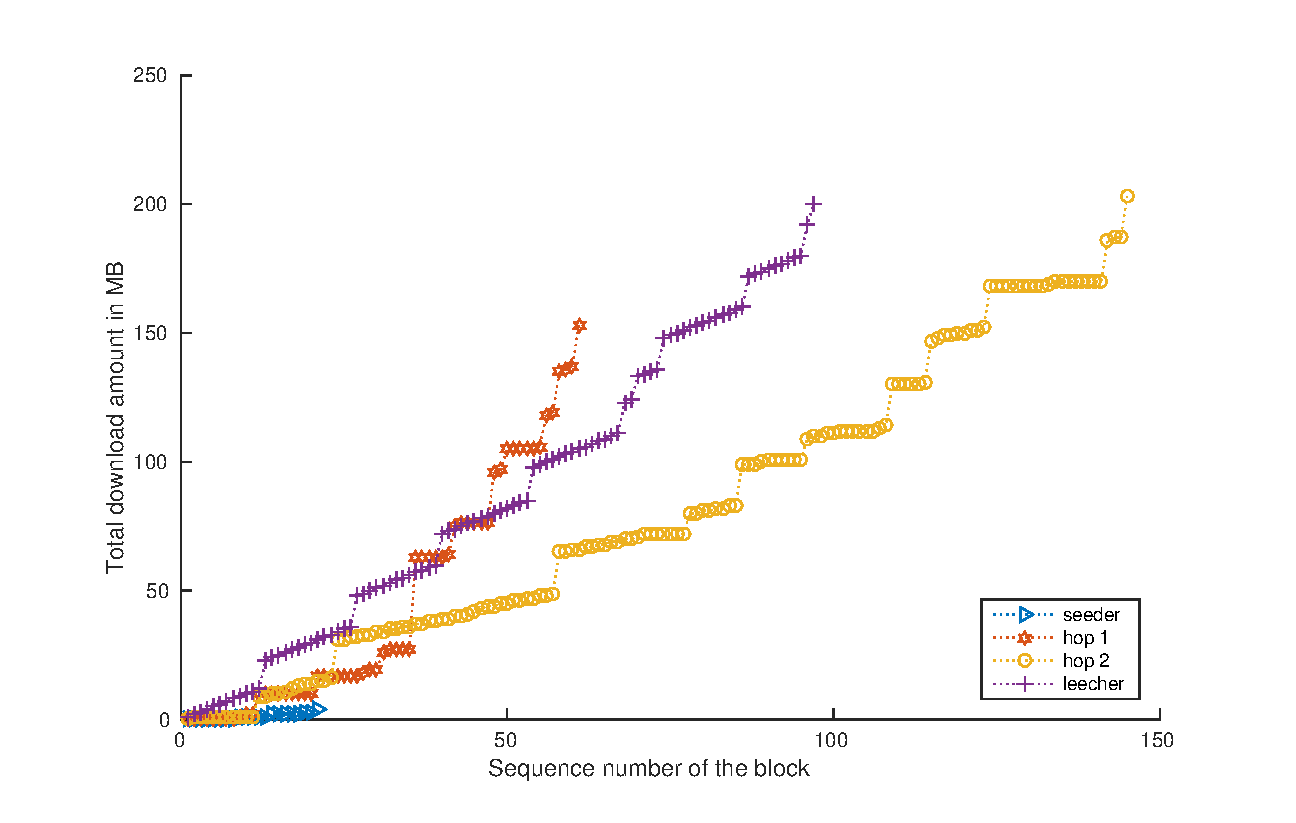
\includegraphics[scale=0.5]{experimentation/anonymous-integrated/integrated-anonymous-down.eps}}
\label{fig:integrated-anonymous-down}
}
\subfigure[Total upload amount.]{
\centerline{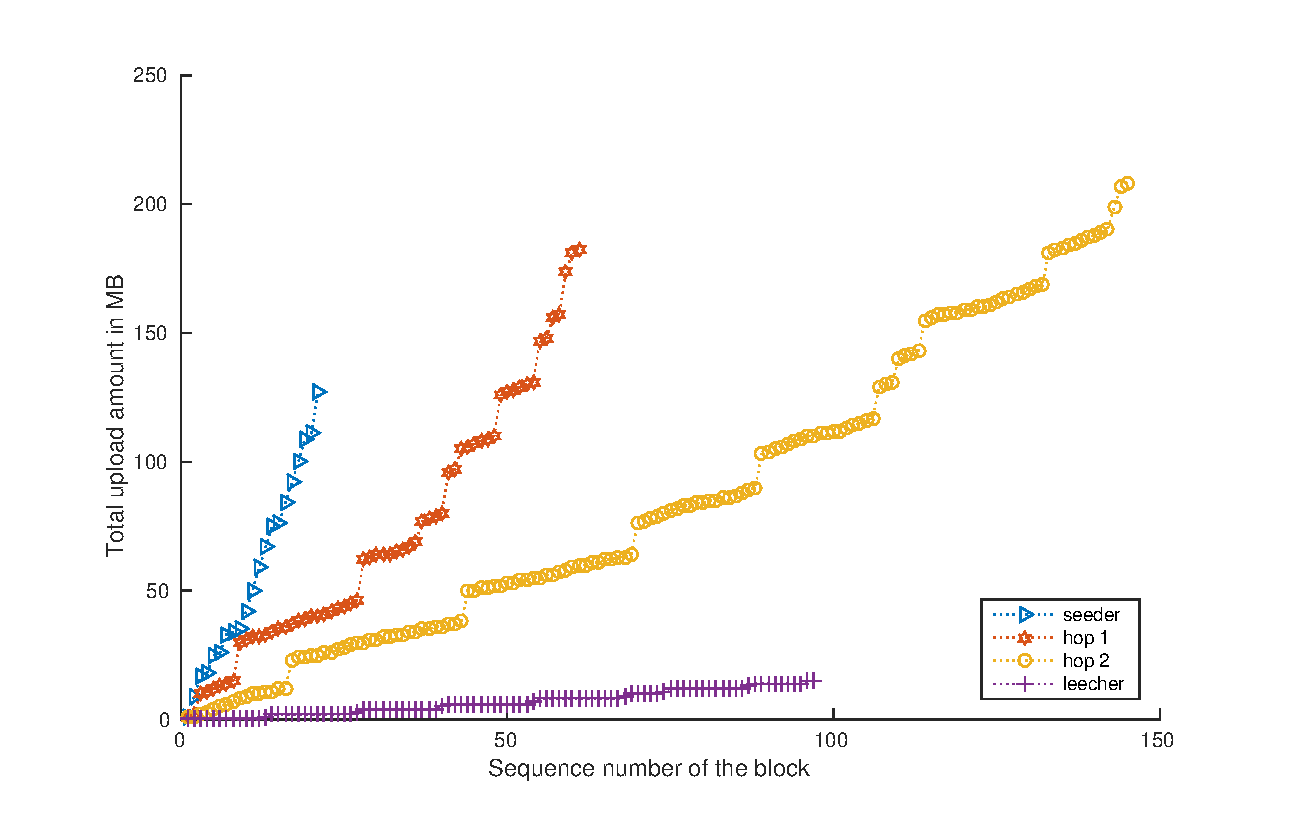
\includegraphics[scale=0.5]{experimentation/anonymous-integrated/integrated-anonymous-up.eps}}
\label{fig:integrated-anonymous-up}
}
\caption{Download and upload amounts during the integrated anonymous download experiment.}
\label{fig:integrated-anonymous-amounts}
\end{figure}

The amount of data that is reported to be transferred is remarkable.
The overhead measures twice the actual download size.
We therefore the conclusion that the integration is not properly and too much data is reported.
It is unclear where this data originates from.

Integrating MultiChain into the anonymous download communities is difficult,
because those communities do not use the standard classes used by Tribler to send messages.
These are necessary to properly integrate MultiChain and a complicated conversion was necessary.
Our recommendation is to refactor the anonymous download communities to use the standard classes
and to make it more clear in the code where data is sent and where data is received.
Also comments should be added to clarify the code.
Currently, there are no comments whatsoever.
This effort should atleast clarify why so much data is reported and will probaly fix the problem.